\documentclass{alex_hü}

\name{Alexander Helbok}
\course{PS Physik}
\hwnumber{4}

\begin{document}
	\renewcommand{\labelenumi}{\alph{enumi})}
	
		
	\section*{20. Wurf von einem Balkon}
		\begin{multicols}{2}
			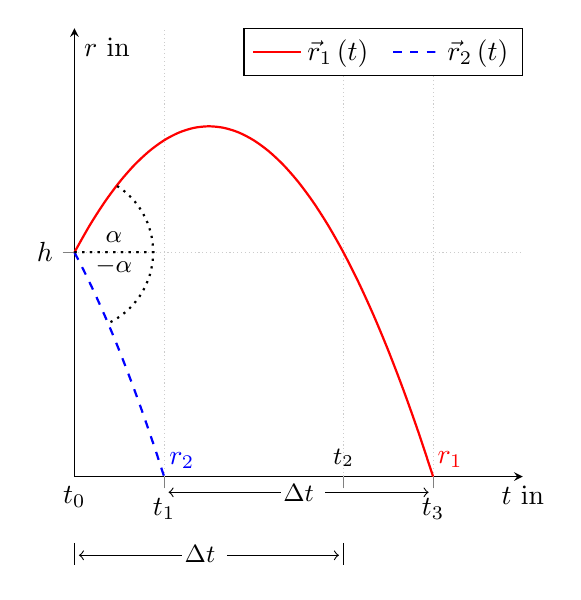
\begin{tikzpicture}
				\begin{axis}[
					clip = false,
					width=207pt,
					height=207pt,
					axis lines=center,
%					axis line style={Stealth-Stealth},
					tick align=outside,
					xmin=0,xmax=2.5,ymin=0,ymax=10,
					xlabel style={below},
					xtick = {0}, ytick = \empty,
					xticklabels={,,},
					yticklabels={,,},
					extra x ticks  = {0.5,2, 1.5},
					extra x tick labels= {$t_1$, $t_3$},
					extra y ticks  = {5},
					extra y tick labels= {$h$},
					xlabel=$t$ in$\si{\s}$,
					ylabel=$r$ in$\si{\m}$,
%					tick label style={font=\tiny},
					grid=major,
					grid style={thin,densely dotted,black!20},
					legend columns=2,
					legend style={at={(axis description cs:1,1)}}]
					\addplot [smooth, thick, red, domain = 0:2] {-5*x^2+7.5*x+5} node[right,pos=0.965]{$r_1$};
					\addplot [smooth, thick, dashed, blue, domain = 0:0.5] {-5*x^2-7.5*x+5} node[right,pos=0.93]{$r_2$};
					\begin{scope}[shift={(0cm,2.85cm)}]
						\draw [dotted, thick](0,0) -- (0:1cm) arc (0:58:1cm);
						\draw (0.5cm,0.185cm) node {\small$\alpha$};
						\draw [dotted, thick](0,0) -- (0:1cm) arc (0:-65:1cm);
						\draw (0.5cm,-0.185cm) node {\small$-\alpha$};
					\end{scope}
					\begin{scope}[shift={(0cm,-0.1cm)}]
						\addplot [<-,  black] coordinates { (0.525,0) (1.15,0)};
						\node at (1.25, -0.2) {\small$\Delta t$};
						\addplot [->,  black] coordinates { (1.4,0) (1.975,0)};
					\end{scope}
					\begin{scope}[shift={(0cm,-0.5cm)}]
						\draw [thin](0,-0.6) -- (0,-1.1);
						\addplot [<-,  black] coordinates { (0.025,0) (0.6,0)};
						\node at (0.7, -0.85) {\small$\Delta t$};
						\addplot [->,  black] coordinates { (0.85,0) (1.475,0)};
						\draw [thin](1.5,-0.6) -- (1.5,-1.1);
					\end{scope}
					\node [below] at (0, 0) {$t_0$};
					\node [above] at (1.5, 0) {\small$t_2$};
					\legend{$ \vec{r}_1\left(t\right)$~~~,$ \vec{r}_2\left(t\right) $}
				\end{axis}
			\end{tikzpicture}\\
			\columnbreak
			\begin{enumerate}
			\item 
			\begin{flalign*}
				\vec{r}_1(t) &= \dl{\vector{v_0\cos(\alpha) t\\ h + v_0\sin(\alpha) t - \tfrac{g}{2}t^2}} &&\\
				\vec{r}_2(t) &= \vector{v_0\cos(-\alpha) t\\ h + v_0\sin(-\alpha) t - \tfrac{g}{2}t^2} &&\\
				r_x(t) &= v_0\cos(\pm\alpha) t &&\\
				r_z(t) &= h + v_0\sin(\pm\alpha) t -\tfrac{g}{2}t^2&&\\[1ex]
				\vec{v}(t) &= \dl{\vector{v_0\cos(\alpha)\\ v_0\sin(\alpha) - gt}} &&\\
				v_x(t) &= v_0\cos(\alpha) &&\\
				v_z(t) &= v_0\sin(\alpha) -gt &&\\[1ex]
			\end{flalign*}
			\end{enumerate}
		\end{multicols}
		\begin{enumerate}
		\setcounter{enumi}{1}
		\item
		\begin{flalign*}
			0 &= r_z(t) &&\\
			0 &= h + v_0\sin\alpha t -\tfrac{g}{2}t^2 &&\\
			t_{i,ii} &= \tfrac{-v_0\sin\alpha \pm \sqrt{v_0\!^2\sin^2\alpha+2gh}}{-g} &&\\
			t_3 &= \dl{\tfrac{-v_0\sin\alpha - \sqrt{v_0\! ^2\sin^2\alpha+2gh}}{-g}} &&\\
		\end{flalign*}
		\item
		\begin{flalign*}
			\left|v_1\right| &= \sqrt{v_x(t_3)^2+v_z(t_3)^2} = \sqrt{\left( v_0\cos\alpha\right) ^2+\left(v_0\sin\alpha-gt_3\right)^2}\ = &&\\
			 &= \sqrt{\left( v_0\cos\alpha\right) ^2+\left(v_0\sin\alpha-g\ \tfrac{v_0\sin\alpha + \sqrt{v_0\!^2 \sin^2\alpha + 2gh}}{g}\right) ^2}\ = &&\\
			 &= \sqrt{v_0\!^2\cos^2\alpha + v_0\!^2\sin^2\alpha + 2gh}\ = &&\\
			 \left|v_1\right| &= \dl{\sqrt{v_0\!^2 + 2gh}} &&
		\end{flalign*}
		\item
		\begin{flalign*}
			r_z(t) &= h &&\\
			h &= h + v_0\sin\alpha t -\tfrac{g}{2}t^2 &&\\
			t_{i,ii} &= \tfrac{-v_0\sin\alpha \pm \sqrt{v_0\!^2\sin^2\alpha}}{-g} &&\\
			t_i &= t_0 = \tfrac{-v_0\sin\alpha + \sqrt{v_0\!^2\sin^2\alpha}}{-g} = 0&&\\
			t_{ii} &= t_3 = \tfrac{-v_0\sin\alpha - \sqrt{v_0\!^2\sin^2\alpha}}{-g} = \tfrac{2v_0\sin\alpha}{g}&&\\[1em]
			\Delta t &= t_3 - t_1 = t_2 - t_0 &&\\
			\Delta t &= \tfrac{2v_0\sin\alpha}{g} - 0 &&\\
			\Delta t &= \dl{\tfrac{2v_0\sin\alpha}{g}} &&
		\end{flalign*}
		\item $\Delta t$ ist die Zeit, die die Kugel mit der steileren Trajektorie braucht, um wieder auf der Starthöhe $h$ zu sein, weil ab dem Zeitpunkt $t_2$ die Bewegungen der zwei Kugeln ident sind. Hierbei ist es egal auf welcher Höhe man startet, da es nicht um den Betrag der Höhe geht, sonder nur darum, wieder auf der anfänglichen Höhe zu sein.
		\end{enumerate}
	
	\section*{21. Golf}

	\begin{enumerate}
		\item $ l = 220 \si{\m},\quad v_0 = 50 \si{\m\per\s},\quad g = 9.81 \si{\m\per\s^2}$
		\begin{multicols}{2}
			\begin{align*}
				&&\vec{r}(t) = \vector{v_0\cos\alpha t\\ v_0\sin\alpha t - \tfrac{g}{2}t^2}\quad \Rightarrow \\ 
			\end{align*}
		\columnbreak 
			\begin{flalign*}
				\\
				x(t) &= v_0\cos\alpha t &&\\
				z(t) &= v_0\sin\alpha t -\tfrac{g}{2}t^2&&
			\end{flalign*}
		\end{multicols}
		\vspace{-2cm}
		\begin{flalign*}
			z(t) &= 0 &&\\
			t_1 &= 0,\quad t_2 = \tfrac{2v_{0}}{g}\sin\alpha &&\\
			x(t_2) &= l = \tfrac{v_{0}\! ^2}{g}\sin2\alpha &&\\
			\alpha &= \tfrac{\arcsin\left(\tfrac{200g}{v_{0}\! ^2} \right)}{2} = \ang{29.84}&&\\
			\alpha_{1,2} &= \ang{45} \pm (\ang{45} - \alpha) &&\\
			\alpha_1 &= \dl{\ang{29.84}},\quad \alpha_2 = \dl{\ang{60.16}} &&
		\end{flalign*}
		\item 
		\begin{flalign*}
			l_{max} &= \tfrac{v_{0}\! ^2}{g} \quad \text{für }\alpha = \ang{45} &&\\
			l_{max} &= \tfrac{50^2 \si{\m}}{9.81 \si{\m\per\s}} = \dl{255 \si{\m}}
		\end{flalign*}
	\end{enumerate}
	\section*{29. Beschleunigte Kreisbewegung}
	\begin{enumerate}
		\item $ \vec{r}(t) = R\ \vector{\cos\gamma t^2\\ \sin\gamma t^2} $
		\begin{flalign*}
			\vec{v}(t) &= \dl{2R\gamma t\ \vector{-\sin\gamma t^2\\ \cos\gamma t^2}} &&\\[1em]
			\left|v(t)\right| &= \sqrt{(2R\gamma t\sin\gamma t^2)^2 + (2R\gamma t\cos\gamma t^2)^2} = &&\\
			\left|v(t)\right| &= \dl{2R\gamma t} && \\[1em]
			s(t) &= R\varphi(t) = \dl{R\gamma t^2} &&
		\end{flalign*}
		\item
		\begin{flalign*}
			\varphi(t) &= \gamma t^2 &&\\
			\omega(t) &= \dl{2\gamma t} &&\\
			\alpha(t) &= \dl{2\gamma} &&
		\end{flalign*}
		\item
		\begin{flalign*}
			\vec{a}(t) &= \dl{\tikzmark{Start1} 2R\gamma\ \vector{-\sin\gamma t^2\\ \cos\gamma t^2} \tikzmark{End1} + \tikzmark{Start2} 4R\gamma^2t^2 \vector{-\cos\gamma t^2\\ -\sin\gamma t^2} \tikzmark{End2}} &&\\[1em]
			\left|a(t)\right| &= \sqrt{(-2R\gamma\sin\gamma t^2 - 4R\gamma^2t^2\cos\gamma t^2)^2 + (2R\gamma\cos\gamma t^2 - 4R\gamma^2t^2\sin\gamma t^2)^2} = &&\\
			\left|a(t)\right| &= \tikzmark{Start3}\sqrt{ 4R^2\gamma^2 \tikzmark{End3} + \tikzmark{Start4} 16R^2\gamma^4 t^4}\tikzmark{End4} &&\\
		\end{flalign*}
		\AddOverBrace[2.2ex]{Start1}{End1}{\scriptsize Tangentialbeschleunigung}
		\AddOverBrace[2.2ex]{Start2}{End2}{\scriptsize Zentripetalbeschleunigung}
		\AddUnderBrace{Start3}{End3}{\scriptsize Tangentialbeschl.}
		\AddUnderBrace{Start4}{End4}{\scriptsize Zentripetalbeschl.}
		\item 
		\begin{multicols}{2}
			\begin{align*}
				4R^2\gamma^2 &< 16R^2\gamma^4 t^4 &&|\ \sqrt{ }\\
				2R\gamma &< 4R\gamma^2 t^2 &&|\ :2R\gamma \\
				1 &< 2\gamma t^2 &&|\ :2\gamma\ |\ \sqrt{}\\
				t &> \dl{\sqrt{\tfrac{1}{2\gamma}}} &&
			\end{align*}
		\columnbreak
		\end{multicols}
		
	für $ t > \frac{1}{\sqrt{2\gamma}} $ liefert die Zentripetalbeschleunigung den Hauptteil der Beschleunigung.
	\end{enumerate}
	
	\newpage
	\section*{31. Zweidimensionale Bahnkurve}
		\begin{multicols}{2}
			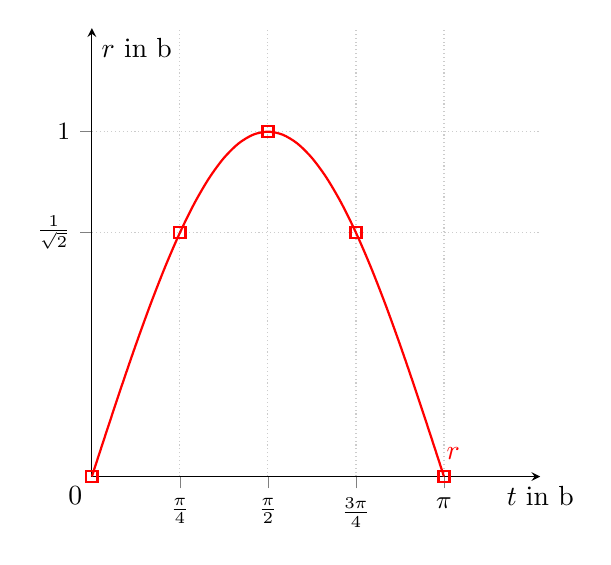
\begin{tikzpicture}
				\begin{axis}[
					clip = false,
					width=207pt,
					height=207pt,
					axis lines=center,
					%					axis line style={Stealth-Stealth},
					tick align=outside,
					xmin=0,xmax=4,ymin=0,ymax=1.3,
					xlabel style={below},
					xtick = {pi/4,pi/2,3*pi/4,pi}, ytick = {1/2^0.5,1},
					xticklabels={$\frac{\pi}{4}$,$\frac{\pi}{2}$,$\frac{3\pi}{4}$,$\pi$},
					yticklabels={$\frac{1}{\sqrt{2}}$,1},
					xlabel=$t$ in b,
					ylabel=$r$ in b,
					tick label style={font=\small},
					grid=major,
					grid style={thin,densely dotted,black!20},
					legend columns=2,
					legend style={at={(axis description cs:1,1)}}]
					\addplot [thick, red, mark=square, only marks]
					plot coordinates {
						(0,0) (pi/4,1/2^0.5) (pi/2,1)
						(3*pi/4,1/2^0.5) (pi,0)
					};
					\addplot [smooth, thick, red, domain = 0:pi] {sin(deg(x))} node[right,pos=0.975]{$r$};
					\node [below left] at (0, 0) {0};
%					\legend{$ \vec{r}_1\left(t\right)$~~~,$ \vec{r}_2\left(t\right) $}
				\end{axis}
			\end{tikzpicture}
			\columnbreak
			\begin{enumerate}
				\item $ \vec{r}(t) = b\ \vector{\omega t\\ \sin\omega t} $
				\begin{flalign*}
					r(t_0) &= \vector{0\\ 0} &&\\
					r(t_1) &= \vector{b\pi/4\\ b/\sqrt{2}} &&\\
					r(t_2) &= \vector{b\pi/2\\ b} &&\\
					r(t_3) &= \vector{3b\pi/4\\ b/\sqrt{2}} &&\\
					r(t_4) &= \vector{\pi\\ 0} &&
				\end{flalign*}
			\end{enumerate}
		\end{multicols}
		\begin{enumerate}
			\setcounter{enumi}{1}
			\item
			\begin{flalign*}
				\vec{v}(t) &= \dl{b\omega\ \vector{1 \\\cos\omega t}} &&\\
				\left|v(t)\right| &= \sqrt{\left(b\omega\right)^2+\left(b\omega\cos\omega t\right)^2} = \dl{b\omega\ \sqrt{1 + \cos^2\omega t}} &&
			\end{flalign*}
			\item
			\begin{flalign*}
				\vec{a}(t) &= \dl{ b\omega^2\ \vector{0 \\-\sin\omega t}} &&\\
				\left|a(t)\right| &= \sqrt{\left(0b\omega^2\right)^2+\left(-b\omega^2\sin\omega t\right)^2} = \dl{b\omega^2\abs{\sin\omega t}} &&
			\end{flalign*}
			\item
			\begin{flalign*}
				\left|a_{\parallel}(t)\right| &= \dv{\left|v(t)\right|}{t} = \dl{-\tfrac{b\omega^2\sin2\omega t}{2\sqrt{1+\cos^2\omega t}}}&&\\[1em]
%				\vec{a}_{\parallel}(t) &= \left|a_{\parallel}(t)\right| \tfrac{\vec{v}(t)}{\left|v(t)\right|} = \left|a_{\parallel}(t)\right| \vec{v}(t) \tfrac{1}{\left|v(t)\right|} = &&\\
%				&= -\tfrac{b\omega^2\sin2\omega t}{2\sqrt{1+\cos^2\omega t}}\ b\omega\ \vector{1 \\\cos\omega t} \tfrac{1}{b\omega\ \sqrt{1 + \cos^2\omega t}} = &&\\
%				\vec{a}_{\parallel}(t) &= \dl{-\tfrac{b\omega^2\sin2\omega t}{2+2\cos^2\omega t}\ \vector{1\\ \cos\omega t}} &&
			\end{flalign*}
			\item
			\begin{flalign*}
%				\vec{a}_{\parallel}(t_1) &= \dl{\vector{-\tfrac{b\omega^2}{3}\\ -\tfrac{b\omega^2}{3\sqrt{2}}}} &&\\[1em]
				\abs{\vec{a}_{\parallel}} &= \sqrt{(-\tfrac{b\omega^2\sin2\omega t_1} {2\sqrt{1+\cos^2\omega t_1}})^2} = \dl{\tfrac{b\omega^2} {\sqrt{6}}} &&\\[1em]
				\left|a_{\perp}(t_1)\right| &= \sqrt{\left|a(t_1)\right|^2 - \left|a_{\parallel}(t_1)\right|^2} = 
				\sqrt{(b\omega^2\sin\omega t_1)^2 - (-\tfrac{b\omega^2\sin2\omega t_1} {2\sqrt{1+\cos^2\omega t_1}})^2} = \sqrt{\tfrac{b^2\omega^4}{2} - \tfrac{b^2\omega^4} {6}} = &&\\
				\left|a_{\perp}(t_1)\right| &= \tfrac{b\omega^2}{\sqrt{3}} &&\\[1em]
				\rho(t_1) &= \tfrac{\left|v(t_1)\right|^2} {\left|a_{\perp}(t_1)\right|} = \tfrac{\left(b\omega\ \sqrt{1 + \cos^2\omega t_1}\right)^2}{\tfrac{b\omega^2}{\sqrt{3}}} = \tfrac{b^2\omega^2\tfrac{3}{2}}{\tfrac{b\omega^2}{\sqrt{3}}} = \tfrac{3\sqrt{3}b^2\omega^2}{2b\omega^2} = &&\\
				\rho(t_1) &= \dl{\tfrac{\sqrt{27}b}{2}} &&
			\end{flalign*}
		\end{enumerate}
\end{document}




